\documentclass[11pt, a4paper]{report}
\usepackage{graphicx, parskip, color, natbib}

% While microtype produces nice results,
% change font size by no more than 1%.
% Need to use lmodern CM fonts in order to scale.
\usepackage{lmodern}
\usepackage[stretch = 10]{microtype}

% Might want to mess with page geometry at some point.
% Handy to have just in case.
\usepackage{geometry}

% Using these packages for vector graphics, e.g. the package
% relationship diagram.
\usepackage{pgf, tikz}
\usetikzlibrary{arrows, positioning, fit, shapes}

% Ensuring we get hyperlinks and that natbib plays nicely with it.
\usepackage{hyperref}
\usepackage{hypernat}

% Defining the file/font/lang formats we want.
\usepackage[utf8]{inputenc}
\usepackage[T1]{fontenc}
\usepackage[english]{babel}

% Requires minted.sty to be in the same directory as this file.
% Also requires pdflatex to be run with -shell-escape, but the makefile
% already does this, use `make all` or `make show`.
% Using the pastie style by default.
\usepackage{minted}
\usemintedstyle{pastie}

% Saving myself from having to format as monospace.
\newcommand{\grid}{\texttt{grid}}
\newcommand{\gridSVG}{\texttt{gridSVG}}
\newcommand{\R}{\texttt{R}}

% Renaming the bibliography section with the name `References`.
\addto{\captionsenglish}{\renewcommand{\bibname}{References}}

% Document properties.
\newcommand{\doctitle}{Web-based Interactive Graphics with gridSVG}
\newcommand{\docauthor}{Simon Potter}
\newcommand{\docdate}{June 19, 2011} % TODO: Change this date later
\title{\doctitle{}}
\author{\docauthor{}}
\date{\docdate{}}
\hypersetup{pdftitle = {\doctitle{} | \docauthor{}},
        	pdfauthor = {\docauthor{}}}

\begin{document}

\begin{titlepage}
\begin{center}

% Space until centre of doc
\vspace*{2.5cm}

% Upper part of the page
\input{images/uoa-logo.pdf_tex}

\vspace{1cm}

% Header text
\textsc{\LARGE University of Auckland} \\[0.4cm]
\textsc{\Large Department of Statistics} \\[1cm]

% Title
\hrule
\vspace{0.1cm} % Not necessary but looks slightly better when closer to the bottom of the box
{\Large \doctitle{}} \\[0.5cm]
\hrule
\vspace{0.5cm}

% Author and supervisor
\begin{minipage}{0.4\textwidth}
\begin{flushleft} \large
\emph{Author:}\\
\docauthor{}
\end{flushleft}
\end{minipage}
\begin{minipage}{0.4\textwidth}
\begin{flushright} \large
\emph{Supervisor:} \\
Dr. Paul Murrell
\end{flushright}
\end{minipage}

% Space until end of page
\vfill

% Bottom of the page
{\large \docdate{}}

\end{center}
\end{titlepage}


\grid{} blah blah \citep{RGraphics} \R{}. blah blah \citet{SVGSpec} \gridSVG{} blah blah \citet{SVGAnnotation}, blah blah blah \citet{gridSVG}.

\begin{center}
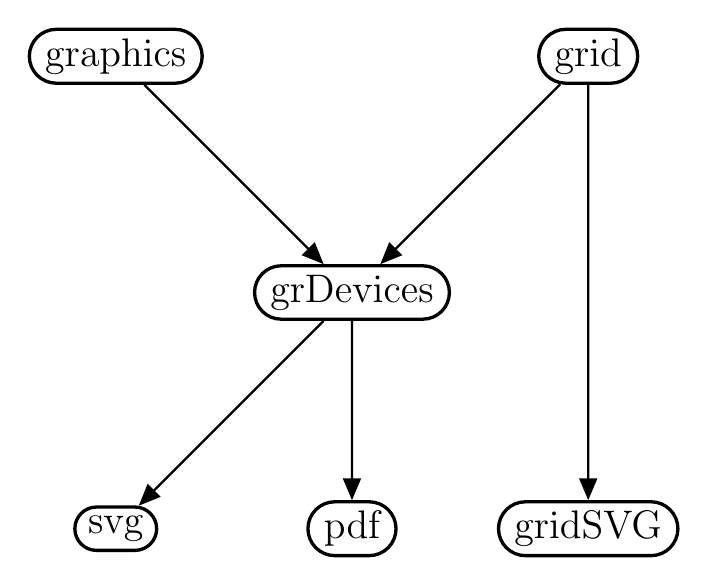
\begin{tikzpicture}[scale=3, >=triangle 45]
\tikzstyle{every node}=[draw,shape=circle];
\node[rounded rectangle, very thick] (grdev) at (1,1)  {\Large grDevices};
\node[rounded rectangle, very thick] (gr) at (0,2) {\Large graphics};
\node[rounded rectangle, very thick] (grid) at (2,2) {\Large grid};
\node[rounded rectangle, very thick] (svg) at (0,0) {\Large svg};
\node[rounded rectangle, very thick] (pdf) at (1,0) {\Large pdf};
\node[rounded rectangle, very thick] (gridsvg) at (2,0) {\Large gridSVG};
\draw [->, thick] (grdev) -- (svg);
\draw [->, thick] (grdev) -- (pdf);
\draw [->, thick] (gr) -- (grdev);
\draw [->, thick] (grid) -- (grdev);
\draw [->, thick] (grid) -- (gridsvg);
\end{tikzpicture}
\end{center}

\begin{minted}[frame=single]{r}
square <- function(x) {
  x * x
}
\end{minted}

\tableofcontents
%\listoffigures
%\listoftables
\begin{abstract}
\thispagestyle{plain} % Ensuring that the abstract's page number appears

Lorem ipsum dolor sit amet, consectetur adipiscing elit. Mauris nec sem metus,
malesuada lacinia erat. Aenean egestas, diam a tempus faucibus, magna sem
ullamcorper nisl, ut molestie tortor nisi vel nisi. Aliquam turpis turpis,
dignissim et ultrices id, laoreet vitae velit. Suspendisse at sollicitudin
augue. Sed molestie aliquet imperdiet. Duis nec dui eu mauris semper sodales.
Sed facilisis arcu eu magna tincidunt imperdiet. Nullam a diam ut sapien porta
scelerisque. Vivamus eget laoreet massa. Duis sit amet nisi eu erat accumsan
tincidunt a eget lorem. Nunc vel massa et nulla ultricies aliquet id at ligula.
Vestibulum ante ipsum primis in faucibus orci luctus et ultrices posuere
cubilia Curae; Suspendisse augue erat, elementum vel venenatis in, viverra ac
mauris. Nullam eget dui et lectus mattis congue sed quis ligula. Phasellus nec
eros tincidunt quam luctus euismod id nec nisl. Maecenas pretium leo in nunc
commodo porta.

\end{abstract}

\chapter{Aim}

The intention of this project is to produce animated and interactive plots on web pages.
These plots can convey more information and be more engaging than regular static graphics.
Currently, the creation of these plots is not possible in \R{} without encountering some difficulty.
A package for \R{} exists that can create the type of plots we want, but it is not capable of producing all but the most basic of statistical graphics.
This package, \gridSVG{}, needed to be improved upon in order to create useful animated and interactive graphics.
The \gridSVG{} package required extending so that it is able to generate plots that are sufficiently similar to those that are produced by \R{}.

\chapter{Introduction}

\section{What are web-based interactive graphics?}

It must be established what are web-based interactive graphics in order to illustrate the intended goal of this project.
Web-based graphics are images that are able to be viewed within a web page by a web browser.
The graphics we intend to produce are not only web-based, but also have the property of being animatable and interactive.
Interactivity involves changing the behaviour or appearance of an image, most commonly by the use of a mouse or keyboard.

\section{Existing solutions}

There are currently a few notable packages for \R{} that do allow for the creation of web-based interactive graphics.
It will be established how these packages work in order to explain why \gridSVG{} is being improved upon.

The \textsf{animation} package can create animated graphics in many formats, including GIF, Flash, and with the use of HTML and JavaScript any common image format can be animated.
In order to produce animated graphics, the \textsf{animation} package generates a series of static plots and pieces them together.
With enough static plots this gives the illusion of animation, much like how a film projector quickly shows a series of static frames when playing a movie.

\textsf{animation} relies heavily on the use of software not present within the package to produce many of the different graphics formats it supports.
In fact, the only formats that do not have any dependencies on third-party software are on-screen animations and HTML pages.
On-screen animations have the drawback of being unable to be stored in any way.
The GIF, Flash, PDF and video formats that \textsf{animation} all require software additional to \R{}.

Other packages have been released but they leverage other graphics systems to implement any animation or interactivity.
These packages include: \textsf{webvis}, which utilises the Protovis Javascript library, \textsf{googleVis}, which uses Google's Visualisation API, and \textsf{gWidgetsWWW} which provides its own Javascript library.
While these systems do all produce animated and interactive graphics, one problem is that they are no longer using \R{} graphics.
This means that a plot that is produced in \R{} will not appear similar to the resulting plots that these packages produce. 

A package that generates animated, interactive graphics via the \R{} graphics system is \textsf{SVGAnnotation} \citet{SVGAnnotation}.
It leverages \R{}'s \texttt{svg()} graphics device by post-processing the output to see which SVG elements correspond with components of a plot.
After performing the post-processing, animation can occur along with interactivity via JavaScript.
It's ability to produce these graphics given the reverse engineering that's required is extraordinary.
However, a significant issue is that while it allows for interesting graphics to be created, the ease at which this can be done is non-trivial.

\section{Motivation for gridSVG}

Here it is discussed why the currently available \R{} packages are not suitable for the construction of web-based interactive graphics.

We deem \textsf{animation} package to be unsuitable for our needs because of the lack of ``true" animation and it's notable dependencies on software that is not packaged.
On top of this, the graphics it creates are likely to be space inefficient compared to a solution that uses true animation.
This is because animation is done through a series of snapshots, rather than a description of the objects and how they are to be animated.

The packages \textsf{webvis}, \textsf{googleVis} and \textsf{gWidgetsWWW} do create the kind of graphics we want, but they use other graphics systems to accomplish this.
We would like to use the facilities \R{} provides with its powerful graphics system to create animated and interactive graphics.
This way we can ensure that the graphics we see in \R{} are what is actually going to be modified when we create our interactive plots.

While \textsf{SVGAnnotation} can create the kind of graphics we desire, it is difficult to understand how it works.
Because of this it is challenging to extend \textsf{SVGAnnotation}'s features to create animated and interactive graphics that are not provided out-of-the-box.

\chapter{The design of gridSVG}

\section{What is grid? How does it work?}

\begin{center}
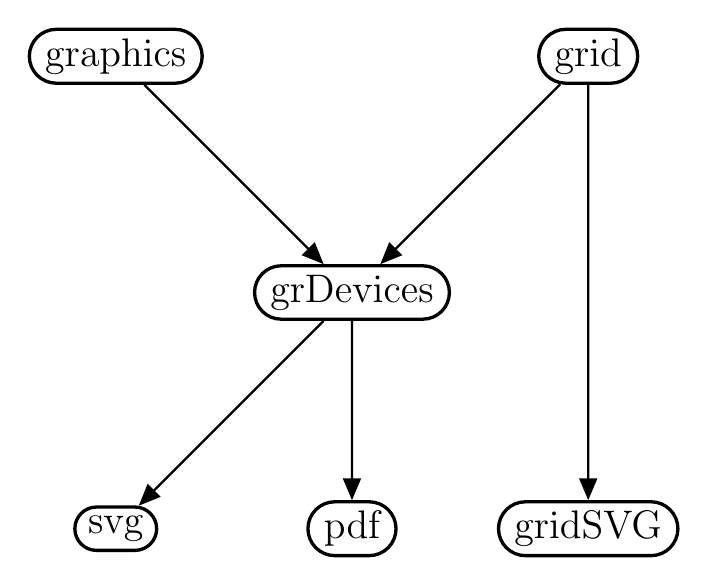
\begin{tikzpicture}[scale=3, >=triangle 45]
\tikzstyle{every node}=[draw,shape=circle];
\node[rounded rectangle, very thick] (grdev) at (1,1)  {\Large grDevices};
\node[rounded rectangle, very thick] (gr) at (0,2) {\Large graphics};
\node[rounded rectangle, very thick] (grid) at (2,2) {\Large grid};
\node[rounded rectangle, very thick] (svg) at (0,0) {\Large svg};
\node[rounded rectangle, very thick] (pdf) at (1,0) {\Large pdf};
\node[rounded rectangle, very thick] (gridsvg) at (2,0) {\Large gridSVG};
\draw [->, thick] (grdev) -- (svg);
\draw [->, thick] (grdev) -- (pdf);
\draw [->, thick] (gr) -- (grdev);
\draw [->, thick] (grid) -- (grdev);
\draw [->, thick] (grid) -- (gridsvg);
\end{tikzpicture}
\end{center}

\section{What is SVG? Javascript?}

\section{Mapping of grid grobs to SVG elements}

\input{./tex/body.tex}
\chapter{Conclusion}

 
\appendix
\input{./tex/appendix.tex}
 
% References:
\clearpage
\addcontentsline{toc}{chapter}{References}
\input{./tex/references.tex}

\bibliographystyle{apa}
\bibliography{references.bib}
\end{document}
